\begin{figure}[h!]
\centering

%% Left: grid-world with a short path highlighted
\begin{subfigure}[t]{0.42\textwidth}
\centering
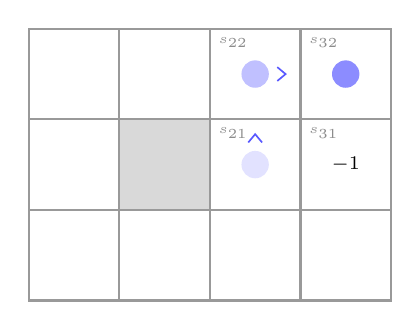
\begin{tikzpicture}[
    cell/.style={minimum size=1.15cm, draw=black!40, thick,
                 font=\scriptsize},
    wall/.style={cell, fill=black!15},
    reward/.style={font=\scriptsize\bfseries},
    agent/.style={circle, fill=blue!45, inner sep=3.5pt},
    ghost/.style={circle, fill=blue!45, inner sep=3.5pt, opacity=0.25},
    slabel/.style={font=\tiny, text=black!45},
]
\def\s{1.15}

% Row 0 (bottom)
\node[cell] (c00) at (0, 0) {};
\node[cell] (c10) at (\s, 0) {};
\node[cell] (c20) at (2*\s, 0) {};
\node[cell] (c30) at (3*\s, 0) {};
% Row 1 (middle)
\node[cell] (c01) at (0, \s) {};
\node[wall] (c11) at (\s, \s) {};
\node[cell] (c21) at (2*\s, \s) {};
\node[cell] (c31) at (3*\s, \s) {};
% Row 2 (top)
\node[cell] (c02) at (0, 2*\s) {};
\node[cell] (c12) at (\s, 2*\s) {};
\node[cell] (c22) at (2*\s, 2*\s) {};
\node[cell] (c32) at (3*\s, 2*\s) {};

% Reward labels (plain black)
\node[reward] at (c32) {$+1$};
\node[reward] at (c31) {$-1$};

% State labels in top-left corner
\node[slabel, anchor=north west] at (c21.north west) {$s_{21}$};
\node[slabel, anchor=north west] at (c22.north west) {$s_{22}$};
\node[slabel, anchor=north west] at (c32.north west) {$s_{32}$};
\node[slabel, anchor=north west] at (c31.north west) {$s_{31}$};

% Agent trail: oldest ghost most faded, recent ghost less faded,
% solid dot at current position
\node[ghost] at (c21) {};
\node[circle, fill=blue!45, inner sep=3.5pt, opacity=0.55] at (c22) {};
\node[agent] at (c32) {};

% Bare chevrons showing direction (no stem)
\draw[semithick, blue!65]
      ([yshift=8pt, xshift=-2.5pt]c21.center) --
      ([yshift=11pt]c21.center) --
      ([yshift=8pt, xshift=2.5pt]c21.center);
\draw[semithick, blue!65]
      ([xshift=8pt, yshift=2.5pt]c22.center) --
      ([xshift=11pt]c22.center) --
      ([xshift=8pt, yshift=-2.5pt]c22.center);

\end{tikzpicture}
\subcaption{Grid-world path: $s_{21} \to s_{22} \to s_{32}$.}
\label{fig:mdp-grid}
\end{subfigure}
\hfill
%% Right: same path as a state-transition graph
\begin{subfigure}[t]{0.52\textwidth}
\centering
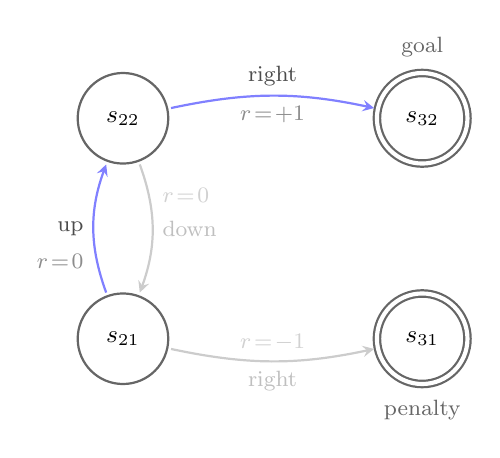
\begin{tikzpicture}[
    state/.style={circle, draw=black!60, thick,
                  minimum size=1.15cm, font=\small},
    terminal/.style={state, double, double distance=1.5pt},
    active/.style={->, thick, >=stealth, blue!50,
                   shorten >=1pt, shorten <=1pt},
    faded/.style={->, thick, >=stealth, black!20,
                  shorten >=1pt, shorten <=1pt},
    alabel/.style={font=\footnotesize, text=black!70},
    rlabel/.style={font=\footnotesize, text=black!45},
    fadea/.style={font=\footnotesize, text=black!25},
    fader/.style={font=\footnotesize, text=black!18},
]

% Nodes -- generous spacing
\node[state]    (s21) at (0, 0)     {$s_{21}$};
\node[state]    (s22) at (0, 2.8)   {$s_{22}$};
\node[terminal] (s32) at (3.8, 2.8) {$s_{32}$};
\node[terminal] (s31) at (3.8, 0)   {$s_{31}$};

% Goal/penalty annotations (plain text)
\node[font=\footnotesize, text=black!60,
      above=2pt] at (s32.north) {goal};
\node[font=\footnotesize, text=black!60,
      below=2pt] at (s31.south) {penalty};

% Active path: s21 -> s22 (up, bent left)
\draw[active] (s21) to[bend left=20]
              node[alabel, left] {up}
              node[rlabel, left, yshift=-12pt] {$r\!=\!0$}
              (s22);

% Active path: s22 -> s32 (right, bent left)
\draw[active] (s22) to[bend left=12]
              node[alabel, above] {right}
              node[rlabel, below] {$r\!=\!+1$}
              (s32);

% Faded: s22 -> s21 (down, bent left)
\draw[faded] (s22) to[bend left=20]
             node[fadea, right] {down}
             node[fader, right, yshift=12pt] {$r\!=\!0$}
             (s21);

% Faded: s21 -> s31 (right, bent right)
\draw[faded] (s21) to[bend right=12]
             node[fadea, below] {right}
             node[fader, above] {$r\!=\!-1$}
             (s31);

\end{tikzpicture}
\subcaption{The same path as a state-transition graph.}
\label{fig:mdp-graph}
\end{subfigure}

\caption{Two views of the same MDP fragment. Left: a path through
  the grid-world from $s_{21}$ to the goal. Right: the same
  states and transitions as a directed graph.}
\label{fig:mdp-views}
\end{figure}
